\section{introduction}

\subsection{workflow}

\begin{figure}
\centering
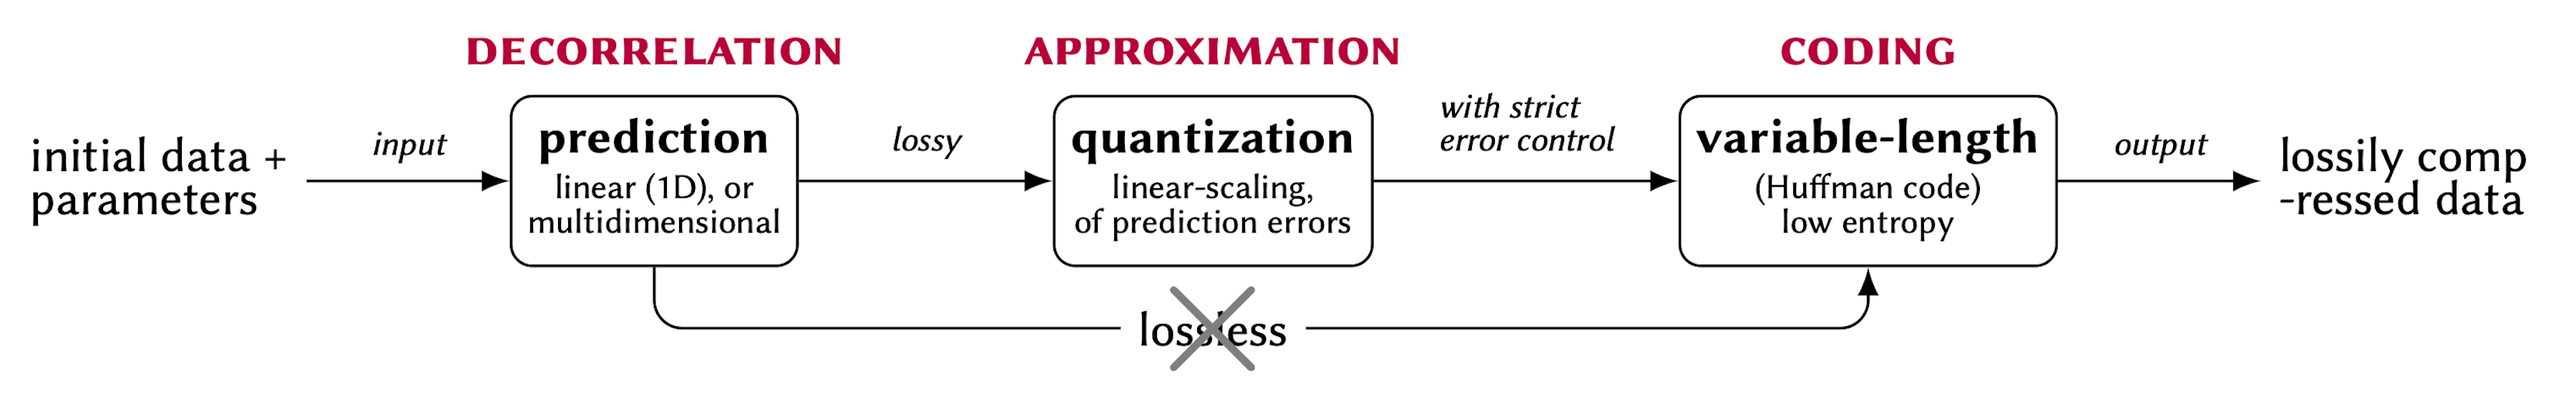
\includegraphics{fig/standalone_errorControl.png}
\caption{Error-control worflow.}
\end{figure}

\subsection{about compression ratio}

\begin{figure}\centering

\begin{tikzpicture}
\node[anchor=east]{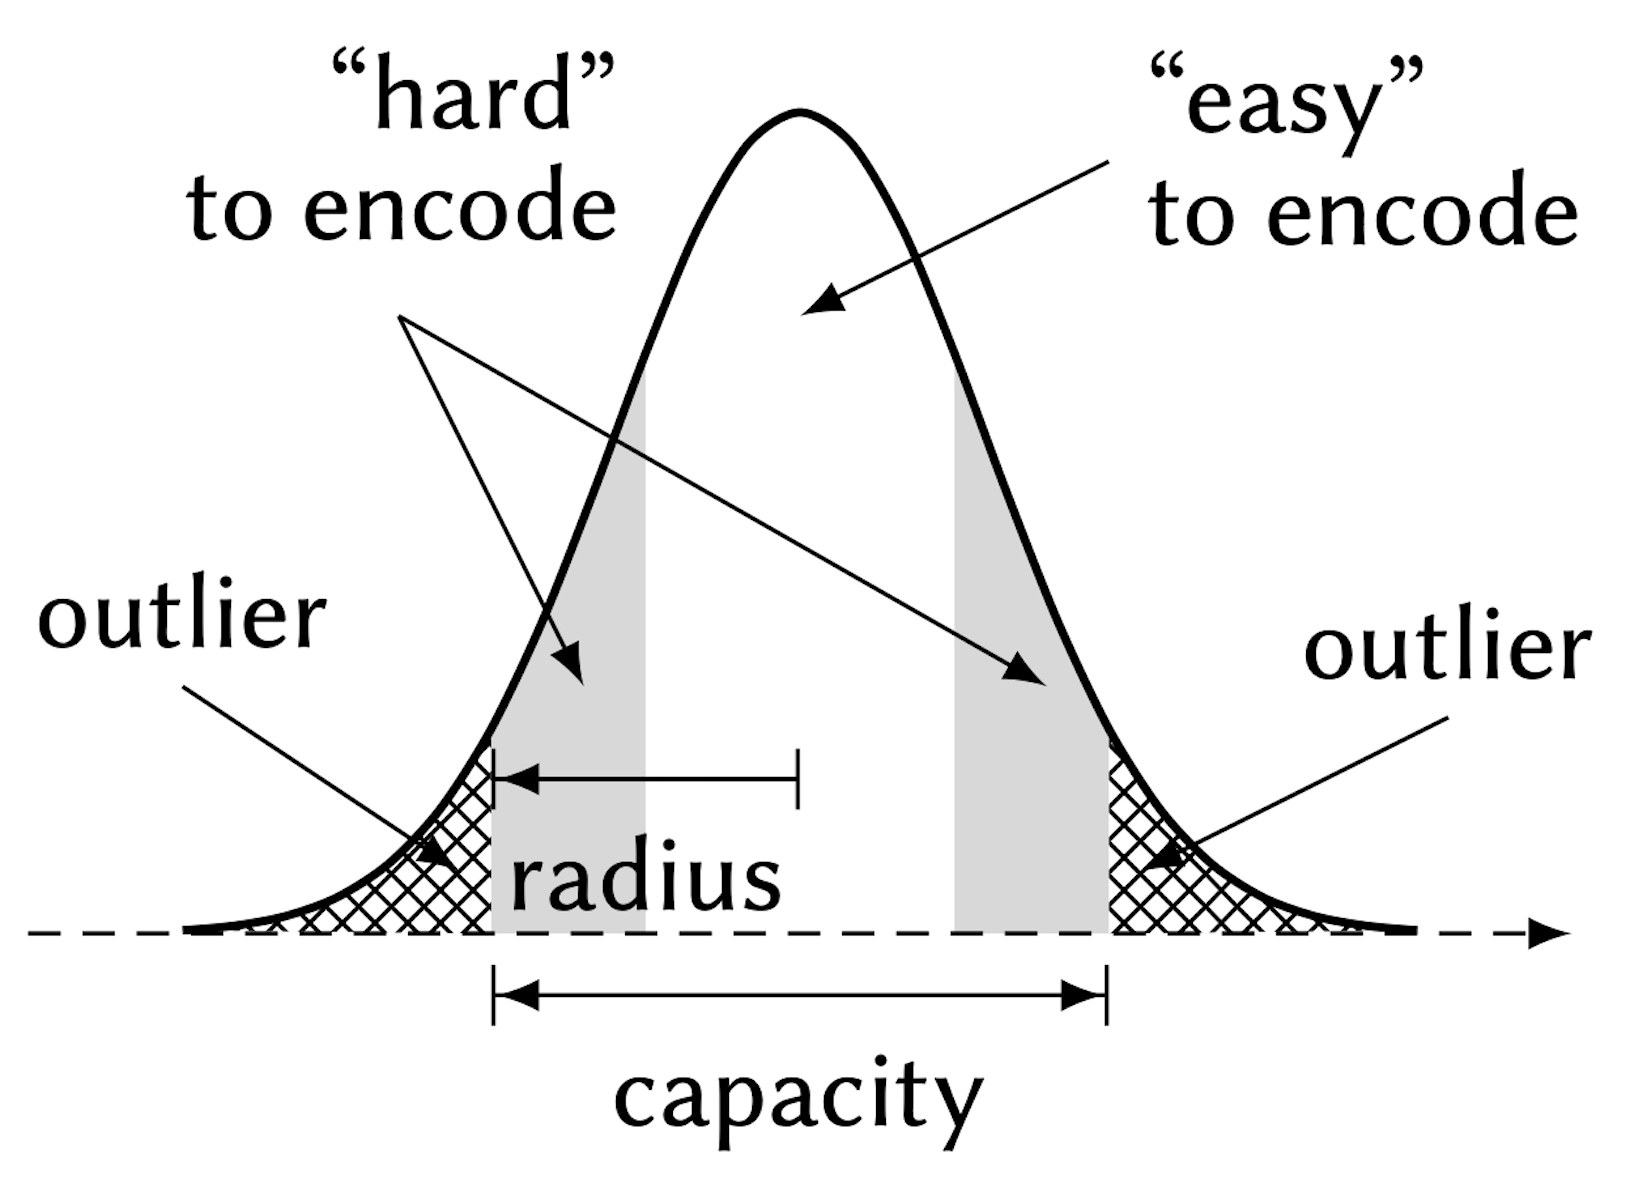
\includegraphics{fig/standalone_demoQcode.png}};
\node[anchor=west]{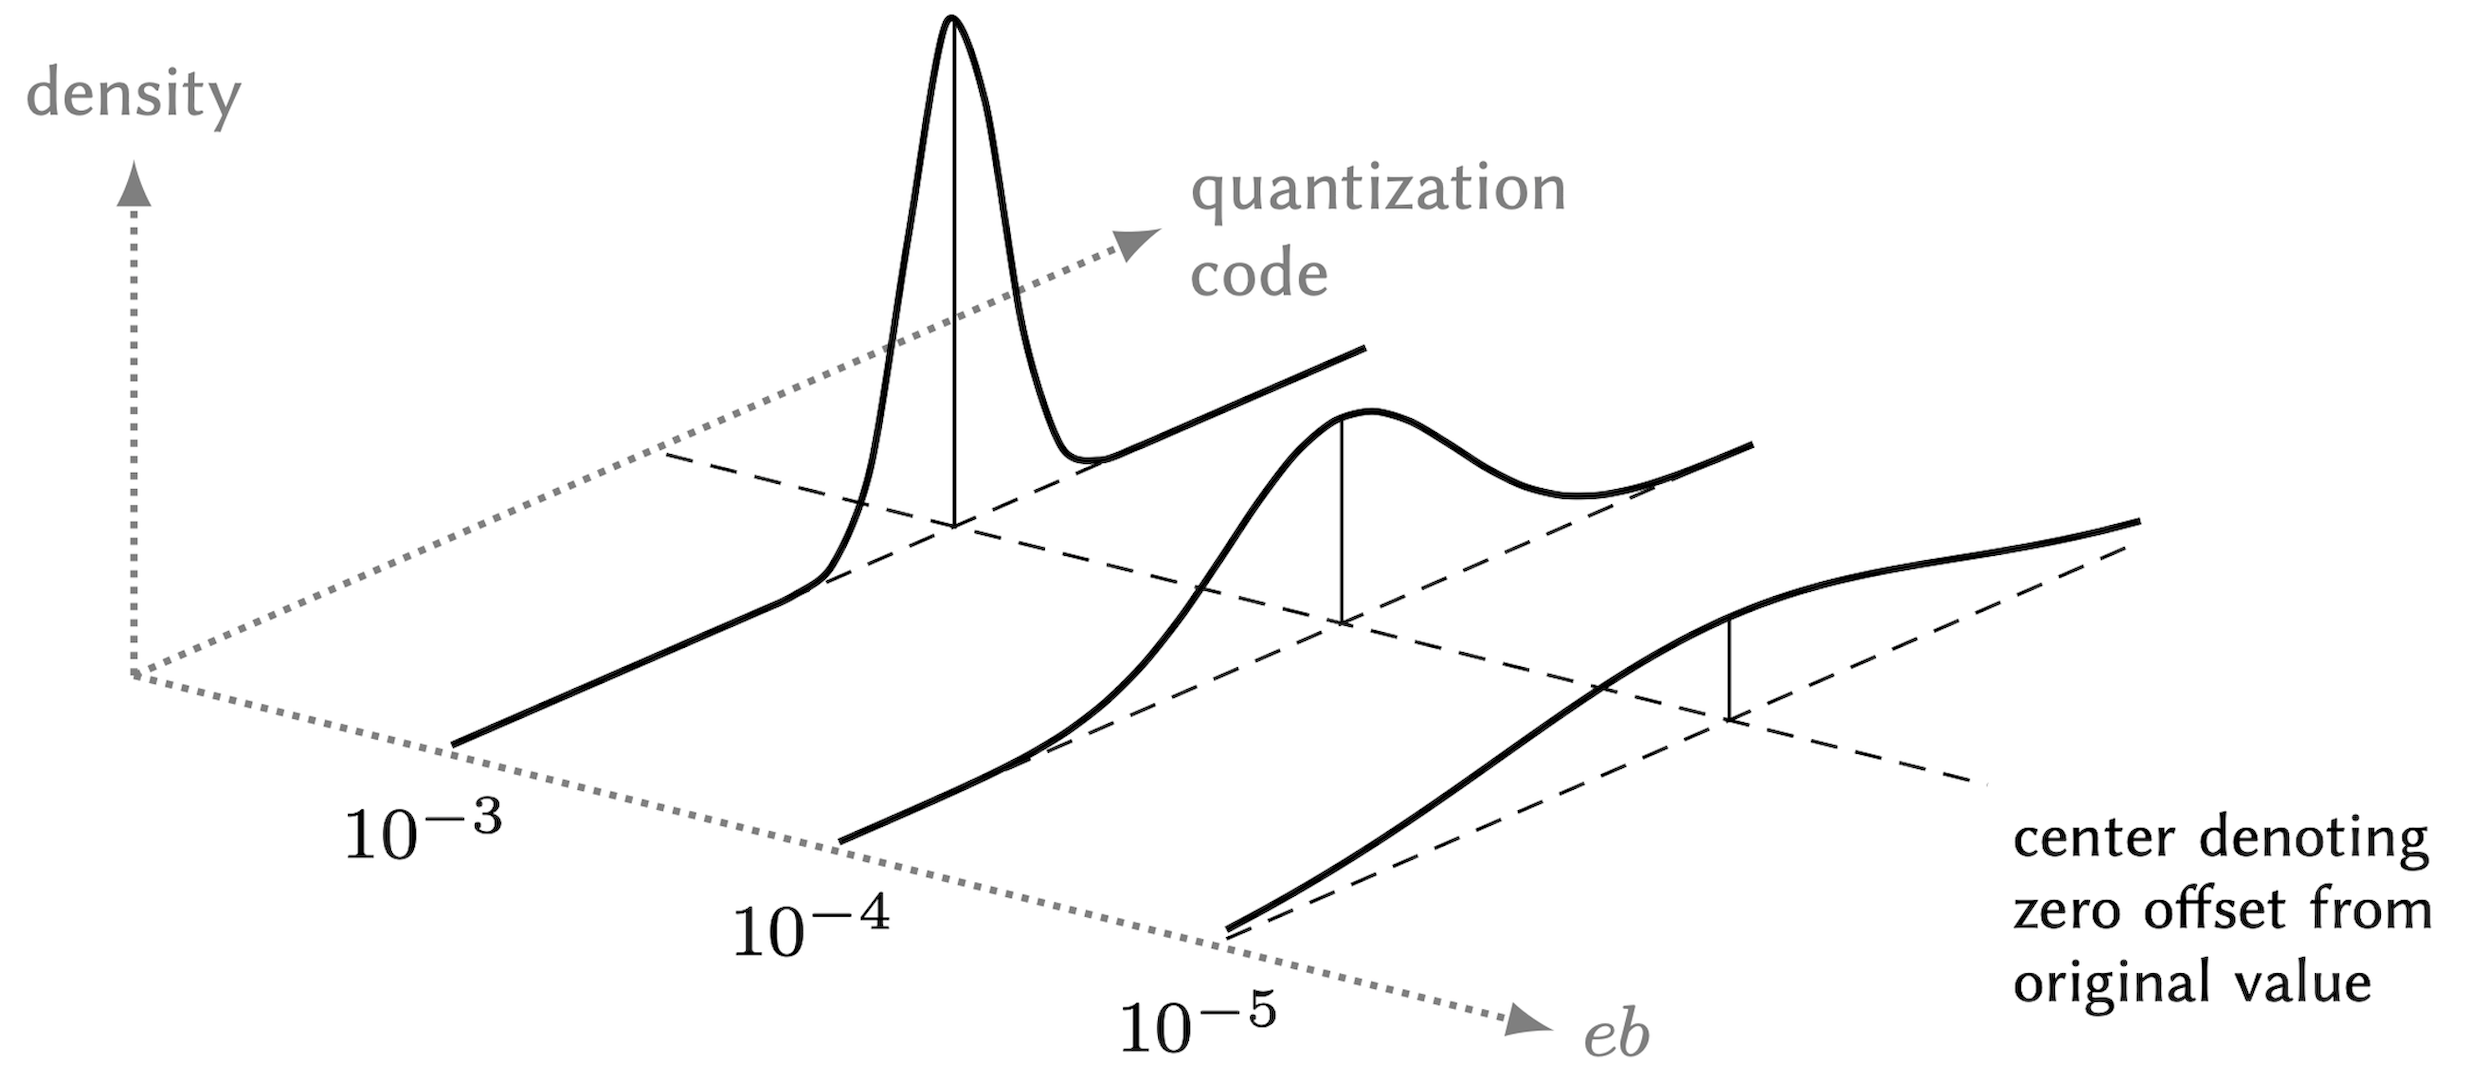
\includegraphics{fig/standalone_demoEb.png}};
\end{tikzpicture}
\caption{(left) classification in prediction error distribution, (right) smaller error bound linear-scales the prediction error distribution.}
\end{figure}

\section{set up}

\subsection{requirements}

\begin{itemize}
\tightlist
\item
  NVIDIA GPU with Kepler, Maxwell, Pascal, Volta, or Turing
  microarchitectures
\item
  CUDA 9.1+ and GCC 7+ (recommended: CUDA 10.1 + GCC 8)
\item
  CMake 3.11+
\end{itemize}

\subsection{download}

\begin{lstlisting}[language=bash]
git clone git@github.com:hipdac-lab/cuSZ.git
\end{lstlisting}

\subsection{compile}

\begin{lstlisting}[language=bash]
cd cuSZ
cmake CMakeLists.txt     # using cmake to compile cuSZ for {1,2,3}-D, with Huffman codec
make
\end{lstlisting}

\section{run}

Commands \passthrough{\lstinline!cusz!} or
\passthrough{\lstinline!cusz -h!} are for instant instructions.

\subsection{\texorpdfstring{\textsc{cuSZ} as a
compressor}{ as a compressor}}

\subsubsection{basic use}

The basic use \textsc{cuSZ} is given below.

\begin{lstlisting}[language=bash]
./cusz -f32 -m r2r -e 1.23e-4.56 -i ./data/sample-cesm-CLDHGH -D cesm -z -x
         ^  ~~~~~~ ~~~~~~~~~~~~~ ~~~~~~~~~~~~~~~~~~~~~~~~~~~~ ~~~~~~~  ^  ^ 
         |   mode   error bound         input datum file        demo   |  |
       dtype                                                   datum  zip unzip
\end{lstlisting}

\passthrough{\lstinline!-D cesm!} specifies preset dataset for
demonstration. In this case, it is CESM-ATM, whose dimension is
1800-by-3600, following \(y\text{-}x\) order. To otherwise specify datum
file and input dimensions arbitrarily, we use
\passthrough{\lstinline!-2 3600 1800!}, then it becomes

\begin{lstlisting}[language=bash]
./cusz -f32 -m r2r -e 1.23e-4.56 -i ./data/sample-cesm-CLDHGH -2 3600 1800 -z -x
\end{lstlisting}

To conduct compression, several input arguments are \textbf{necessary},

\begin{itemize}
\tightlist
\item
  \passthrough{\lstinline!-z!} or \passthrough{\lstinline!--zip!} to
  compress
\item
  \passthrough{\lstinline!-x!} or \passthrough{\lstinline!--unzip!} to
  decompress
\item
  \passthrough{\lstinline!-m!} or \passthrough{\lstinline!--mode!} to
  speciry compression mode. Options include
  \passthrough{\lstinline!abs!} (absolute value) and
  \passthrough{\lstinline!r2r!} (relative to value range).
\item
  \passthrough{\lstinline!-e!} or \passthrough{\lstinline!--eb!} to
  specify error bound
\item
  \passthrough{\lstinline!-i!} to specify input datum file
\item
  \passthrough{\lstinline!-D!} to specify demo dataset name or
  \passthrough{\lstinline!-\{1,2,3\}!} to input dimensions
\end{itemize}

\subsubsection{tuning}

There are also internal a) quant. code representation, b) Huffman
codeword representation, and c) chunk size for Huffman coding exposed.
Each can be specified with argument options.

\begin{itemize}
\item
  \passthrough{\lstinline!-Q!} or \passthrough{\lstinline!--quant-rep!}
  or \passthrough{\lstinline!--bcode-bitwidth <8|16|32>!} to specify
  bincode/quant. code representation. Options 8, 16, 32 are for
  \passthrough{\lstinline!uint8\_t!},
  \passthrough{\lstinline!uint16\_t!},
  \passthrough{\lstinline!uint32\_t!}, respectively. (Manually
  specifying this may not result in optimal memory footprint.)
\item
  \passthrough{\lstinline!-H!} or
  \passthrough{\lstinline!--huffman-rep!} or
  \passthrough{\lstinline!--hcode-bitwidth <32|64>!} to specify Huffman
  codeword representation. Options 32, 64 are for
  \passthrough{\lstinline!uint32\_t!},
  \passthrough{\lstinline!uint64\_t!}, respectively. (Manually
  specifying this may not result in optimal memory footprint.)
\item
  \passthrough{\lstinline!-C!} or
  \passthrough{\lstinline!--huffman-chunk!} or
  \passthrough{\lstinline!--hcode-chunk [256|512|1024|...]!} to specify
  chunk size for Huffman codec. Should be a power-of-2 that is
  sufficiently large. (This affects Huffman decoding performance
  \emph{significantly}.)
\end{itemize}

\subsubsection{extension and use scenarios}

\paragraph{preprocess}

Some application such as EXAFEL preprocesses with binning \footnote{A
  current binning setting is to downsample a 4-by-4 cell to 1 point.} in
addition to skipping Huffman codec.

\paragraph{disabling modules}

Also according to EXAFEL, given binning and
\passthrough{\lstinline!uint8\_t!} have already result in a compression
ratio of up to 16, Huffman codec may not be expected in a real-world use
scenario. In such cirumstances, \passthrough{\lstinline!--skip huffman!}
can be used.

Other module skipping for use scenarios are in development.

\subsection{\texorpdfstring{\textsc{cuSZ} as an analytical
tool}{ as an analytical tool}}

\passthrough{\lstinline!--dry-run!} or \passthrough{\lstinline!-r!} in
place of \passthrough{\lstinline!-a!} and/or
\passthrough{\lstinline!-x!} enables dry-run mode to get PSNR. This
employs the feature of dual-quantization that the decompressed data is
guaranteed the same with prequantized data.

\subsection{example}

\begin{enumerate}
\def\labelenumi{\arabic{enumi}.}
\item
  run a 2D CESM demo at 1e-4 relative to value range

\begin{lstlisting}[language=bash]
./cusz -f32 -m r2r -e 1e-4 -i ./data/sample-cesm-CLDHGH -D cesm -z -x
\end{lstlisting}
\item
  alternatively, to use full option name,

\begin{lstlisting}[language=bash]
./cusz -f32 --mode r2r --eb 1e-4 --input ./data/sample-cesm-CLDHGH \
    --demo cesm --zip --unzip
\end{lstlisting}
\item
  run a 3D Hurricane Isabel demo at 1e-4 relative to value range

\begin{lstlisting}[language=bash]
./cusz -f32 -m r2r -e 1e-4 -i ./data/sample-hurr-CLOUDf48 -D huricanne -z -x
\end{lstlisting}
\item
  run CESM demo with 1) \passthrough{\lstinline!uint8\_t!}, 2) 256
  quant. bins,

\begin{lstlisting}[language=bash]
./cusz -f32 -m r2r -e 1e-4 -i ./data/sample-cesm-CLDHGH -D cesm -z -x \
    -d 256 -Q 8
\end{lstlisting}
\item
  in addition to the previous command, if skipping Huffman codec,

\begin{lstlisting}[language=bash]
./cusz -f32 -m r2r -e 1e-4 -i ./data/sample-cesm-CLDHGH -D cesm -z -x \
    -d 256 -Q 8 --skip huffman  # or `-X/-S huffman`
\end{lstlisting}
\item
  some application such as EXAFEL preprocesses with binning \footnote{A
    current binning setting is to downsample a 4-by-4 cell to 1 point.}
  in addition to skipping Huffman codec

\begin{lstlisting}[language=bash]
./cusz -f32 -m r2r -e 1e-4 -i ./data/sample-cesm-CLDHGH -D cesm -z -x \
    -d 256 -Q 8 --pre binning --skip huffman    # or `-p binning`
\end{lstlisting}
\item
  dry-run to get PSNR and to skip real compression or decompression;
  \passthrough{\lstinline!-r!} also works alternatively to
  \passthrough{\lstinline!--dry-run!}

\begin{lstlisting}[language=bash]
./cusz -f32 -m r2r -e 1e-4 -i ./data/sample-cesm-CLDHGH -D cesm --dry-run   # or `-r`
\end{lstlisting}
\end{enumerate}

\section{project management}

\subsection{TODO List}

Please refere to
\href{https://github.com/hipdac-lab/cuSZ/projects/2}{\emph{Project
Management page}}.

\subsection{\texorpdfstring{\texttt{changelog}}{changelog}}

May, 2020

\begin{description}
\tightlist
\item[perf]
{[}need review{]} decrease memory footprint by merging
\passthrough{\lstinline!data!} and \passthrough{\lstinline!ourlier!}
during compression
\item[feature]
add \passthrough{\lstinline!--skip huffman!} and
\passthrough{\lstinline!--verify huffman!} options
\item[feature]
add binning as preprocessing, \passthrough{\lstinline!--pre binning!} or
\passthrough{\lstinline!-p binning!}
\item[prototype]
use \passthrough{\lstinline!cuSparse!} to transform
\passthrough{\lstinline!outlier!} to dense format
\item[feature]
add \passthrough{\lstinline!argparse!} to check and parse argument
inputs
\item[refactor]
add CUDA wrappers (e.g., \passthrough{\lstinline!mem::CreateCUDASpace!})
\end{description}

April, 2020

\begin{description}
\tightlist
\item[feature]
add concise and detailed help doc
\item[deploy]
\passthrough{\lstinline!sm\_61!} (e.g., P1000) and
\passthrough{\lstinline!sm\_70!} (e.g., V100) binary
\item[feature]
add dry-run mode
\item[refactor]
merge \textsc{cuSZ} and Huffman codec in driver program
\item[perf]
1D \passthrough{\lstinline!PdQ!} (and reverse
\passthrough{\lstinline!PdQ!}) \passthrough{\lstinline!blockDim!} set to
32, throughput changed from 2.7 GBps to 16.8 GBps
\item[deploy]
histograming, 2013 algorithm supersedes naive 2007 algorithm by default
\item[feature]
add communication of equivalance calculation
\item[feature]
use cooperative groups (CUDA 9 required) for canonical Huffman codebook
\item[perf]
faster initializing shared memory for PdQ, from 150 GBps to 200 GBps
\item[feature]
add Huffman inflating/decoding
\item[refactor]
merge \{1,2,3\}-D \textsc{cuSZ}
\item[feature]
set 32- and 64-bit as internal Huffman codeword representation
\item[feature]
now use arbitrary multiple-of-8-bit for quant. code
\item[feature]
switch to canonical Huffman code for decoding
\end{description}

March, 2020

\begin{description}
\tightlist
\item[perf]
tuning thread number for Huffman deflating and inflating
\item[feature]
change freely to 32bit intermediate Huffman code representation
\item[demo]
add EXAFEL demo
\item[feature]
switch to faster histograming
\end{description}

February, 2020

\begin{description}
\tightlist
\item[demo]
SDRB suite metadata in \passthrough{\lstinline!SDRB.hh!}
\item[feature]
visualize histogram (\passthrough{\lstinline!pSZ!})
\item[prototype]
add CPU \textsc{pSZ}, p for prototyping
\item[milestone]
\passthrough{\lstinline!PdQ!} for compression, Huffman encoding and
deflating
\end{description}

\section{reference}

\begin{description}
\tightlist
\item[{[}1{]}]
Gómez-Luna, Juan, José María González-Linares, José Ignacio Benavides,
and Nicolás Guil. ``An optimized approach to histogram computation on
GPU.'' Machine Vision and Applications 24, no. 5 (2013): 899-908.
\item[{[}2{]}]
Barnett, Mark L. ``Canonical Huffman encoded data decompression
algorithm.'' U.S. Patent 6,657,569, issued December 2, 2003.
\end{description}

\section{acknowledgement}

This R\&D was supported by the Exascale Computing Project (ECP), Project
Number: 17-SC-20-SC, a collaborative effort of two DOE organizations --
the Office of Science and the National Nuclear Security Administration,
responsible for the planning and preparation of a capable exascale
ecosystem. This repository was based upon work supported by the U.S.
Department of Energy, Office of Science, under contract
DE-AC02-06CH11357, and also supported by the National Science Foundation
under Grant No.~1948447.

\section{license}

\begin{verbatim}
BSD 3-Clause License

Copyright (c) 2020, Jiannan Tian, Dingwen Tao, Sheng Di, Franck Cappello
All rights reserved.

cuSZ - A GPU Accelerated Error-Bounded Lossy Compressor for Scientific Data
[Version 0.1]

Redistribution and use in source and binary forms, with or without
modification, are permitted provided that the following conditions are met:

1. Redistributions of source code must retain the above copyright notice, this
   list of conditions and the following disclaimer.

2. Redistributions in binary form must reproduce the above copyright notice,
   this list of conditions and the following disclaimer in the documentation
   and/or other materials provided with the distribution.

3. Neither the name of the copyright holder nor the names of its
   contributors may be used to endorse or promote products derived from
   this software without specific prior written permission.

THIS SOFTWARE IS PROVIDED BY THE COPYRIGHT HOLDERS AND CONTRIBUTORS "AS IS"
AND ANY EXPRESS OR IMPLIED WARRANTIES, INCLUDING, BUT NOT LIMITED TO, THE
IMPLIED WARRANTIES OF MERCHANTABILITY AND FITNESS FOR A PARTICULAR PURPOSE ARE
DISCLAIMED. IN NO EVENT SHALL THE COPYRIGHT HOLDER OR CONTRIBUTORS BE LIABLE
FOR ANY DIRECT, INDIRECT, INCIDENTAL, SPECIAL, EXEMPLARY, OR CONSEQUENTIAL
DAMAGES (INCLUDING, BUT NOT LIMITED TO, PROCUREMENT OF SUBSTITUTE GOODS OR
SERVICES; LOSS OF USE, DATA, OR PROFITS; OR BUSINESS INTERRUPTION) HOWEVER
CAUSED AND ON ANY THEORY OF LIABILITY, WHETHER IN CONTRACT, STRICT LIABILITY,
OR TORT (INCLUDING NEGLIGENCE OR OTHERWISE) ARISING IN ANY WAY OUT OF THE USE
OF THIS SOFTWARE, EVEN IF ADVISED OF THE POSSIBILITY OF SUCH DAMAGE.

Contact: Dingwen Tao (dingwen.tao@ieee.org), Jiannan Tian(tian.jn09@gmail.com)
\end{verbatim}
